\documentclass[english,margin=2pt]{standalone}
\usepackage{babel}
\usepackage[utf8]{inputenc}
\usepackage{helvet}
\renewcommand{\rmdefault}{\sfdefault}
\usepackage[T1]{fontenc}
\usepackage[version=4]{mhchem} % \ce{CO2}
\usepackage{tikz}
\usetikzlibrary{arrows.meta,calc,positioning,shapes}

% Colors
% greys
\definecolor{jdlightestgrey}{HTML}{ECECEC}
\definecolor{jdverylightgrey}{HTML}{B3B3B3}
\definecolor{jdlightergrey}{HTML}{999999}
\definecolor{jdlightgrey}{HTML}{808080}
\definecolor{jdgrey}{HTML}{666666}
\definecolor{jddarkgrey}{HTML}{4D4D4D}
\definecolor{jddarkergrey}{HTML}{333333}
\definecolor{jddarkestgrey}{HTML}{1A1A1A}

% blues
\definecolor{jddarkestblue}{HTML}{0B1728}
\definecolor{jddarkerblue}{HTML}{162D50}
\definecolor{jddarkblue}{HTML}{214478}
\definecolor{jdblue}{HTML}{5F8DD3}
\definecolor{jdlightblue}{HTML}{87AADE}
\definecolor{jdlighterblue}{HTML}{AFC6E9}
\definecolor{jdlightestblue}{HTML}{D7E3F4}

% green
\definecolor{jdgreen}{HTML}{00AA44}

% others
\definecolor{jdblack}{HTML}{050505}
\definecolor{jdwhite}{HTML}{FFFFFF}

% commodities
\definecolor{co2}{RGB}{160, 160, 160}
\definecolor{elec}{RGB}{255, 170, 0}
\definecolor{gas}{RGB}{128, 64, 0}
\definecolor{grid}{RGB}{0,119,138}
\definecolor{heat}{RGB}{230, 112, 36}
\definecolor{solar}{RGB}{243, 174, 0}

\begin{document}

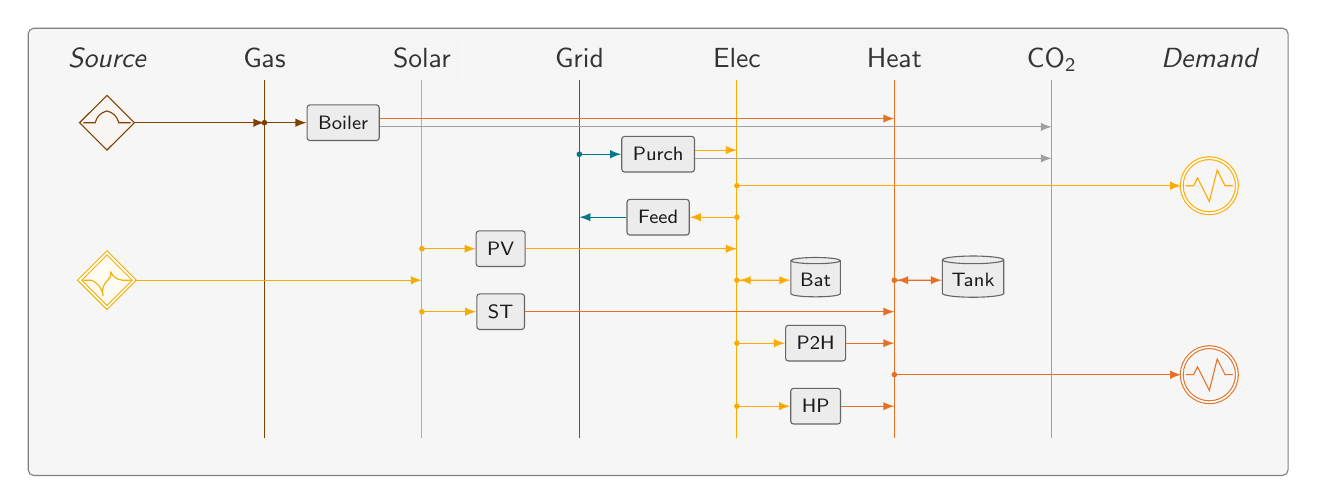
\begin{tikzpicture}[
  input/.style={latex-{Circle[length=2pt]}, shorten >= -1pt},
  output/.style={-latex},
  commodity/.style={text=jddarkergrey, fill=jdlightergrey!10},
  supdem/.style={text=jddarkergrey, font=\itshape},
  process/.style={draw=jdgrey, text=jddarkestgrey, fill=jdlightestgrey, rounded corners=1pt, align=center, inner sep=4pt, font=\scriptsize},
  storage/.style={draw=jdgrey, text=jddarkestgrey, fill=jdlightestgrey, cylinder, shape border rotate=90, aspect=0.125, font=\scriptsize},
  biconn/.style={latex-{latex[]Circle[length=2pt]},shorten >= -1pt},
  demand/.style={draw, circle, double, minimum size=0.7cm},
  supim/.style={draw, diamond, double, minimum size=0.7cm,aspect=1.5},
  stock/.style={draw, diamond, minimum size=0.7cm, aspect=2},
  site/.style={draw=jdlightgrey, fill=jdlightestgrey!45, rounded corners=2pt},
  stockpic/.pic={\draw (-3mm,0) to (-1.5mm,0) to [bend left] (0,1.5mm) to [bend left] (1.5mm,0) to (3mm,0);}, 
  supimpic/.pic={\draw (-3mm,0) to (-2mm,0) to [bend left] (-.5mm,-2mm) to [bend left] (.1mm,0) to [bend right] (.5mm,1mm) to [bend right] (2mm,0) to (3mm,0);},
  demandpic/.pic={\draw[scale=.1] (-3,0) -- ++(1,0) -- ++(.5,1) -- ++(.5,-1) -- ++(1,-2) -- ++(1,4) -- ++(1,-2) -- ++(1,0);}
]
\coordinate (dx) at (1cm, 0);
\coordinate (dy) at (0, 0.8cm);
\coordinate (do) at (0, 3pt);
\foreach \column /\commodity in {0/left, 1/gas, 2/solar, 3/grid, 4/elec, 5/heat, 6/co2, 7/right}
  \foreach \row in {0,1,2,3,4,5,6}
    \coordinate (\commodity\row) at ($2*\column*(dx)-\row*(dy)$);

% site
\draw[site] ($(left0.north west)-(dx)+.5*(dy)$) 
  rectangle ($(right6.south east)+(dx)-.6*(dy)$);

% commodity lines & labels
\begin{scope}[text height=1.5ex, text depth=.25ex]
\draw (left0) node[supdem] {Source};
\draw[gas] (gas0) node[commodity] {Gas} -- (gas6);
\draw[solar] (solar0) node[commodity] {Solar} -- (solar6);
\draw[grid] (grid0) node[commodity] {Grid} -- (grid6);
\draw[elec] (elec0) node[commodity] {Elec} -- (elec6);
\draw[heat] (heat0) node[commodity] {Heat} -- (heat6);
\draw[co2] (co20) node[commodity] {\ce{CO2}} -- (co26);
\draw (right0) node[supdem] {Demand};
\end{scope}

% processes
\node[process] (boiler) at ($ (gas1)+(dx) $) {Boiler}
  edge[gas,input] (gas1);
  \path ($ (boiler.east)+0.5*(do) $) edge[heat,output] ($ (heat1)+0.5*(do) $);
  \path ($ (boiler.east)-0.5*(do) $) edge[co2,output] ($ (co21)-0.5*(do) $);
\node[process] (pv) at ($ (solar3)+(dx) $) {PV}
  edge[solar,input] (solar3)
  edge[elec,output] (elec3);
\node[process] (st) at ($ (solar4)+(dx) $) {ST}
  edge[solar,input] (solar4)
  edge[heat,output] (heat4);
\node[process]  (purch) at ($ (grid2)+(dx)+.5*(dy) $) {Purch}
  edge[grid,input] ($ (grid2)+.5*(dy) $);
  \path ($ (purch.east)+.5*(do) $) edge[elec,output] ($ (elec2)+.5*(dy)+.5*(do) $);
  \path ($ (purch.east)-.5*(do) $) edge[co2,output] ($ (co22)+.5*(dy)-.5*(do) $);
\node[process] (feedin) at ($ (grid2)+(dx)-.5*(dy) $) {Feed}
  edge[elec,input] ($ (elec2)-.5*(dy) $)
  edge[grid,output] ($ (grid2)-.5*(dy) $);
\node[process] (heatrod) at ($ (elec5) + (dx) + .5*(dy) $) {P2H}
  edge[elec,input] ($ (elec5) + .5*(dy) $)
  edge[heat,output] ($ (heat5) + .5*(dy) $);
\node[process] (heatpump) at ($ (elec6) + (dx) + .5*(dy) $) {HP}
  edge[elec,input] ($ (elec6) + .5*(dy) $)
  edge[heat,output] ($ (heat6) + .5*(dy) $);

% storage
\node[storage] (bat) at ($(elec3)+(dx)-.5*(dy)$) {Bat}
  edge[biconn,elec] ($ (elec3) -.5*(dy) $);
\node[storage] (tank) at ($(heat3)+(dx)-.5*(dy)$) {Tank}
  edge[biconn,heat] ($ (heat3) -.5*(dy) $);

% demand
\node[demand,elec] (elec demand) at (right2) {}
  edge[input,elec] (elec2); 
\pic at (elec demand) [elec] {demandpic};
\node[demand,heat] (heat demand) at ($ (right5) $) {}
  edge[input,heat] ($ (heat5) $);
\pic at (heat demand) [heat] {demandpic};

% supply
\node[stock, gas, fill=gas!5] (gas supply) at (left1) {}
  edge[output,gas] (gas1);
  \pic at (gas supply) [draw=gas] {stockpic};
\node[supim,solar,fill=solar!5] (solar supply) at  ($ (left3) - 0.5*(dy) $) {}
  edge[output,solar] ($ (solar3) - 0.5*(dy) $);
  \pic at (solar supply) [draw=solar] {supimpic};
\end{tikzpicture}

\end{document}
